% \documentclass[journal]{vgtc}                % final (journal style)
\documentclass[review,journal]{vgtc}         % review (journal style)
%\documentclass[widereview]{vgtc}             % wide-spaced review
%\documentclass[preprint,journal]{vgtc}       % preprint (journal style)
%\documentclass[electronic,journal]{vgtc}     % electronic version, journal

%% Uncomment one of the lines above depending on where your paper is
%% in the conference process. ``review'' and ``widereview'' are for review
%% submission, ``preprint'' is for pre-publication, and the final version
%% doesn't use a specific qualifier. Further, ``electronic'' includes
%% hyperreferences for more convenient online viewing.

%% Please use one of the ``review'' options in combination with the
%% assigned online id (see below) ONLY if your paper uses a double blind
%% review process. Some conferences, like IEEE Vis and InfoVis, have NOT
%% in the past.

%% Please note that the use of figures other than the optional teaser is not permitted on the first page
%% of the journal version.  Figures should begin on the second page and be
%% in CMYK or Grey scale format, otherwise, colour shifting may occur
%% during the printing process.  Papers submitted with figures other than the optional teaser on the
%% first page will be refused.

%% These three lines bring in essential packages: ``mathptmx'' for Type 1
%% typefaces, ``graphicx'' for inclusion of EPS figures. and ``times''
%% for proper handling of the times font family.

\usepackage{mathptmx}
\usepackage{graphicx}
\usepackage{times}

\usepackage{placeins}
\usepackage{dingbat}
\usepackage{pifont}
\newcommand{\xmark}{\ding{55}}%

%% We encourage the use of mathptmx for consistent usage of times font
%% throughout the proceedings. However, if you encounter conflicts
%% with other math-related packages, you may want to disable it.

\usepackage{color,soul}

%% This turns references into clickable hyperlinks.
\usepackage[bookmarks,backref=true,linkcolor=black]{hyperref} %,colorlinks
\hypersetup{
  pdfauthor = {},
  pdftitle = {},
  pdfsubject = {},
  pdfkeywords = {},
  colorlinks=true,
  linkcolor= black,
  citecolor= black,
  pageanchor=true,
  urlcolor = black,
  plainpages = false,
  linktocpage
}

%% If you are submitting a paper to a conference for review with a double
%% blind reviewing process, please replace the value ``0'' below with your
%% OnlineID. Otherwise, you may safely leave it at ``0''.
\onlineid{0}

%% declare the category of your paper, only shown in review mode
\vgtccategory{Research}

%% allow for this line if you want the electronic option to work properly
\vgtcinsertpkg

%% In preprint mode you may define your own headline.
%\preprinttext{To appear in IEEE Transactions on Visualization and Computer Graphics.}

%% Paper title.

%Make sure to use a non-STAR title -AGF
\title{A Taxonomy of Visualization Tasks and Requirements for the Effective Analysis of Biological Pathways}

%% This is how authors are specified in the journal style

%% indicate IEEE Member or Student Member in form indicated below
\author{Paul Murray, Francesco Paduano, and Angus Forbes}
\authorfooter{
%% insert punctuation at end of each item
\item
 Paul Murray is a PhD student at the University of Illinois at Chicago's Electronic Visualization Lab. E-mail: pmurra5@uic.edu
}

%other entries to be set up for journal
\shortauthortitle{Murray \MakeLowercase{\textit{et al.}}: STAR Report}
%\shortauthortitle{Firstauthor \MakeLowercase{\textit{et al.}}: Paper Title}

\newcounter{task}
\newcounter{requirement}

\newcommand*{\p}[1]{\paragraph{\textbf{#1}}}
\newcommand*{\tasklabel}[1]{\refstepcounter{task}\thetask\label{#1}}
\newcommand*{\reqlabel}[1]{\refstepcounter{requirement}\therequirement\label{#1}}


%% Abstract section.
\abstract{
Understanding complicated networks of interactions and chemical components is essential to solving contemporary problems in modern biology, especially in domains such as cancer and systems research. In these domains, biological pathway data is used to represent chains of interactions that occur within a given biological process. Visual representations can help researchers understand and interact with complex pathway data in a number of ways. Here, we present a taxonomy of tasks that are regularly performed by researchers who work with biological pathway data. These tasks were generated from interviews with several domain experts. From these tasks we generate a set of requirements that should be taken into consideration when designing pathway visualization software. We then perform a review of visualization techniques that are used in the visualization of complex pathway data. We also perform a survey of a variety of pathway visualization tools that utilize different visualization techniques. We conclude with a discussion of future work that is motivated by comments received from domain experts.
} % end of abstract

%% Keywords that describe your work. Will show as 'Index Terms' in journal
%% please capitalize first letter and insert punctuation after last keyword
\keywords{Biological visualization}

%% ACM Computing Classification System (CCS). 
%% See <http://www.acm.org/class/1998/> for details.
%% The ``\CCScat'' command takes four arguments.

\CCScatlist{ % not used in journal version
%  \CCScat{K.6.1}{Management of Computing and Information Systems}%
% {Project and People Management}{Life Cycle};
%  \CCScat{K.7.m}{The Computing Profession}{Miscellaneous}{Ethics}
}

%% Uncomment below to include a teaser figure.
   \teaser{
   \centering
%   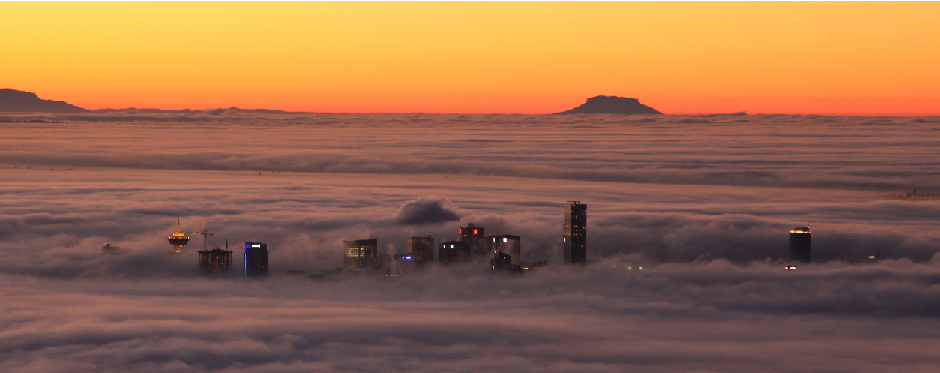
\includegraphics[width=16cm]{CypressView}
%   \caption{In the Clouds: Vancouver from Cypress Mountain.}
  }

%% Uncomment below to disable the manuscript note
%\renewcommand{\manuscriptnotetxt}{}

%% Copyright space is enabled by default as required by guidelines.
%% It is disabled by the 'review' option or via the following command:
% \nocopyrightspace

%%%%%%%%%%%%%%%%%%%%%%%%%%%%%%%%%%%%%%%%%%%%%%%%%%%%%%%%%%%%%%%%
%%%%%%%%%%%%%%%%%%%%%% START OF THE PAPER %%%%%%%%%%%%%%%%%%%%%%
%%%%%%%%%%%%%%%%%%%%%%%%%%%%%%%%%%%%%%%%%%%%%%%%%%%%%%%%%%%%%%%%%

\begin{document}

%% The ``\maketitle'' command must be the first command after the
%% ``\begin{document}'' command. It prepares and prints the title block.

%% the only exception to this rule is the \firstsection command
\firstsection{Introduction}

\maketitle

Understanding complicated networks of interactions and chemical components is essential to solving contemporary problems in modern biology, especially in domains such as cancer and systems research~\cite{hanahan2011hallmarks}. In order to limit the scope of their analyses, researchers often work with \emph{pathways}, which are used to describe a chain of interactions between biochemical and biological entities within a cell. Pathways are small, curated subsets of a much larger, complex graph of interactions between molecules, and a given pathway usually represents a particular biological process that is relevant within some research context. For example, Figure \ref{fig:kvik} shows a typical representation of a pathway as a human-curated node-link diagram, where nodes are biological entities and edges represent interactions between them.

\begin{figure}[htb]
  \centering
  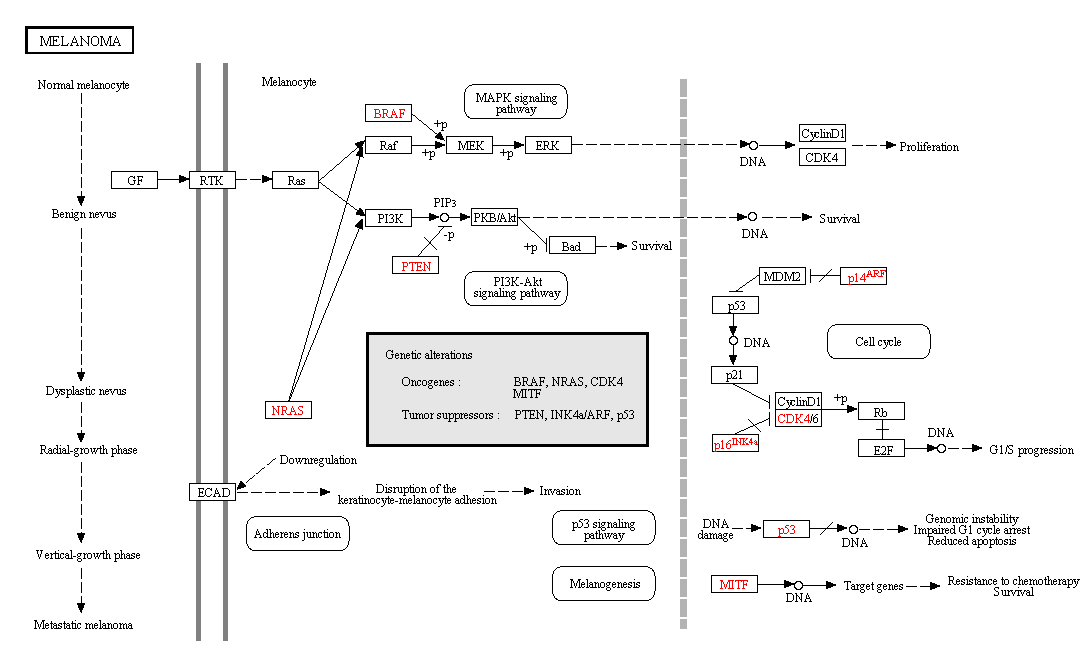
\includegraphics[width=\linewidth]{figures/kegg2}
  \caption{\label{fig:kvik} A view of a typical KEGG diagram. From~\cite{Fjukstad2014kvik}.}
\end{figure}

%\p{Pathways are very complex}

Researchers who work with pathway data are confronted with a number of challenges. Pathway files may contain hundreds of proteins and biomolecules that participate in a variety of reactions. In an abstract sense, reactions can be seen as state transitions with multiple inputs and outputs. Participants --- genes, proteins, and other molecules within a cell --- can act as inputs or outputs to multiple reactions, and the relationships between reactions inherently include feedback loops. Reactions often have an effect on other reactions, inhibiting or promoting their frequency. These molecular activation pathways are inherently dynamic, which limits the utility of any static graph representation \cite{kitano2002systems}. Representing complexity while also enabling researchers to see higher order patterns is a significant challenge \cite{saraiya2005visualizing}.

%\p{Pathways are useful for presentation}

Pathway diagrams can be useful for both presentation and analysis. For presentation, pathway diagrams can contextualize a set of biological processes within a cell, and diagrams often show the location of cellular membranes in order to help provide a frame of reference for a given process. Ideally, a pathway diagram allows a viewer to efficiently understand a complex set of biological relationships.

%\p{Pathways are useful for analysis}

While pathways may be useful for presenting and contextualizing a set of reactions, they can also be an important part of analyses in domains related to molecular biology and systems research, among others.

%\p{Domain context}

For example, molecular activation pathways are of critical importance to cancer researchers, who hope to understand --- and potentially disrupt --- malignant cycles of uncontrolled cellular growth, replication, and mediated cell death \cite{cairns2011regulation}. Effective cancer drug development involves determining how proteins affected by a drug in turn affect important cellular pathways, and in this domain the downstream consequences of a particular drug effect are especially important \cite{luo2003targeting}. In a separate domain, stem-cell researchers work with pathways that will precipitate a desired cellular differentiation into specific cell types \cite{reya2001stem}.

%\p{Static representations are not enough}

In the last decade, analyses that involve hundreds or thousands of genes and gene products have become common. When analyzing such large and complex data, visual representations can be essential. Often, static representations are inadequate. The complexity and amount of information that needs to be incorporated in given diagram can make static representations cluttered and difficult to interpret. Thus, modern tools make careful use of user interactions and visualization techniques to allow a user to effectively explore and analyze pathway data.

%\p{Designing effective tools}

Designing effective visual analytics applications requires a detailed understanding of analysis tasks that are performed by the user. Pathway data are often large and complex, and analysts will want to perform a variety of tasks depending on their research domain. Tasks may be exploratory in nature, and a useful visualization of pathway data could reveal new insights to a researcher. Tasks may also involve detailed queries or calculations of various network metrics, for example. A comprehensive understanding of tasks performed by domain researchers in a typical analysis is essential to the design and implementation of an effective visual analytics application.

%\p{Other reviews}

Here we perform a comprehensive analysis of tasks and requirements in an effort to design effective platforms for visual analytics of pathway data. Previous reviews of pathway analysis tools~\cite{Gehlenborg2010omics,Suderman2007tools} have surveyed the population of available applications. However, the most recent review was published over five years ago, and it includes only a surface-level discussion of tasks, requirements, and visual encoding techniques.

%\p{In this work}

In this work, we present a description and analysis of tasks and requirements related to biological pathway research. Tasks were gathered from several interviews with domain experts who work with biological pathway data. After an introduction to the structure and content of pathway data, we describe the tasks that were garnered from our interviews. Using these tasks, we then describe the high-level requirements of an effective visual analytics platform for pathway data. We then review visual representations of pathway data in the context of our requirements. We also review existing tools that implement those visual representations. Finally, avenues of future research are considered, along with a brief summary of lessons learned from domain experts.

\subsection{Pathway data}

In order to aid an understanding of pathway visualization tools, an understanding of the structure of pathway data structures is necessary. In this section we briefly explain the structure of typical pathway data files. 

\subsubsection{Pathway Data Model}

Information stored in any pathway data file can generally be broken down into three components:

\begin{itemize}

\item \textbf{Entity}\\
An entity is a component of a pathway such as a gene, a gene product (i.e. a protein), a complex of proteins, or a small biomolecule within a cell. Entities are identified by name and are involved in one or more relationships. Importantly, pathways themselves can be entities within other pathways.
\item \textbf{Relationship}\\
A relationship involves two or more entities. Various kinds of relationships which different biological meanings are present in a pathways. Relationships can be directed or undirected, and they can involve more than two entities.
\item \textbf{Meta-data}\\
The complex nature of the information stored in a pathway requires additional data to be stored with each entity and relationship. Meta-data can include experimental data, scientific information such as the molecular structure of a chemical compound, as well as links to additional resources or publications related to an entity or relationship.

\end{itemize}


\subsubsection{Pathway Data Formats}

Pathway data can be stored in one of several file formats. In particular \textit{BioPAX}~\cite{demir2010biopax}, \textit{KEGG}~\cite{kanehisa2000kegg} and \textit{SBML} are the most popular standards for storing the complex data structure described in the previous section. These formats are XML based and represent data as an ontology. \emph{BioPAX}, in particular, was designed to be a general format for biological pathways across a variety of domain contexts~\cite{demir2010biopax}.

Other formats are employed for the visualization of biological pathways that are not specific to the field of biology. For instance \textit{SIF Simple Interaction Format} used by \textit{Cytoscape}~\cite{Shannon2003cytoscape} is used to visualize undirected interactions between participants.

\section{Interviews}

\begin{table*}[htb]
%% Table captions on top in journal version
 \caption{Researchers Interviewed}
 \label{vis_accept}
 \scriptsize
 \begin{center}
   \begin{tabular}{p{0.5cm}p{5cm}p{10cm}}
     Code & Position & Domain \\
   \hline
     NH 
     & Distinguished Professor, \newline Biochemistry and Molecular Genetics 
     & Mechanisms of cell survival, cell cycle control, metabolism, and genesis of cancer.
     \\ % Nissim Hay
     QW 
     & Assistant Professor, \newline Biochemistry and Molecular Genetics 
     & Proteomics, epigenetic maintenance of adult heart function.
     \\ % Qun-Tian Wang
     GY
     & Assistant Professor, \newline Molecular and Cellular Biology
     & Systems and computational biology.
     \\ % Guang Yao
     RG
     & Assistant Professor, \newline Molecular and Cellular Biology
     & Systems and computational biology.
     \\ % Ryan Gutenkunst
     DF
     & Postdoctoral Research Associate, \newline Biochemistry and Molecular Genetics
     & High throughput gene expression analysis.
     \\ % Damiano Fantini
     FZ
     & Researcher, \newline Molecular Oncology
     & Cancer research
     \\ % Federica Zill
     AJ
     & Master's Student
     & Bioinformatics
     \\ % Ankit Jambusaria
    \label{table:interviews}
   \end{tabular}
 \end{center}
\end{table*}

Interviews were conducted with seven biological scientists, each of whom works with pathway data in some form. Information on each of the researchers we interviewed is presented in Table~\ref{table:interviews}. Throughout this text, interviewers are identified by a two letter code found in Table~\ref{table:interviews}. Those interviewed included one tenured professor, three assistant professors, one researcher at a cancer research institution, one postdoctoral research associate, and one masters student in bioinformatics. Interviews were loosely structured, but interview questions were designed to elicit a detailed understanding of the tasks performed by the researcher in a typical analysis, as well as an understanding of the type and structure of data that each researcher worked with. Each researcher also presented their views on the utility of pathway data and pathway diagrams in general.

\section{Tasks}

Drawing on our interviews with domain experts, here we compile a list of tasks relevant to biological pathway analysis. Task descriptions can be found in Table 

\begin{table}[h]

\caption{List of tasks}

\begin{tabular}{p{0.5cm}p{7cm}}
\hline
code & description \\
\hline
T1 & Examine   the   upstream   and   downstream   connections between two entities within a pathway.\\
T2 & Understand   complex   relationships   of   activation   and inhibition between multiple entities.\\
T3 & Detect feedback loops of activation and inhibition within a pathway.\\
T4 & Examine  high-level  relationships  between  modules  and pathways\\
T5 & Discover processes that are upstream or downstream of a given set of entities, and vice versa.\\
T6 & Understand the hierarchical structure of protein complexes.\\
T7 & Analyze high-throughput \emph{omics} data.\\
T8 & Discover potential ``causal'' mechanisms of up- or down-regulation within a set of entities.\\
T9 &  Simulate the effects of activation,  inhibition,  or knockout within a pathway.\\
T10 & Incorporate new entities or relationships into an existing pathway and examine their effects.\\
T11 & Incorporate experimental results with pathway data.\\
T12 & Curate, edit, construct, and “debug” pathway data files. \\
T13 & Reveal levels of confidence or uncertainty associated with relationships within a pathway. \\
\hline

\label{table:tasks}

\end{tabular}

\end{table}

% \subsection{Tasks related to connections between individual entities, pathways, and processes}

Understanding how entities within pathways are connected was of critical importance to all of the researchers we interviewed, and is essential to most research related to pathway data. While some analyses involve undirected relationships between genes or gene products, studies of metabolic networks and other inter-cellular processes rely on directed relationships, and several researchers that we interviewed stressed the importance of understanding directed relationships between entities. 

When discussing directed paths between entities, one entity is said to be \emph{upstream} or \emph{downstream} of another. As mentioned earlier, understanding upstream and downstream relationships is particularly important to domains such as cancer drug research, where a drug may affect a small subset of genes or gene products, which in turn will affect various downstream processes.

In most cases, a directed relationship is meant to represent a biochemical reaction, where one entity is consumed as a reactant and another is produced as a product. Thus, an upstream entity may be connected to a downstream entity through a chain of several directed links. In the most basic sense, the ``entities'' mentioned above are genes, gene products (such as proteins or complexes), or other small molecules within a cell. A researcher may be interested in understanding the path of reactions (or other relationships) that connects two entities.
\ \\

\textbf{Task \tasklabel{task:upstreamDownstreamEntities}} Examine the upstream and downstream connections between two entities within a pathway.
\ \\

It is important to note, however, that directed relationships in biological pathways can take a variety of forms, such as entities that that modulate --- \emph{inhibit} or \emph{activate} --- the catalysis of other biochemical reactions~\cite{demir2010biopax}. All of the researchers interviewed stressed the importance of understanding these modular relationships within a pathway.
\ \\

\textbf{Task \tasklabel{task:activateInhibit}} Understand complex relationships of activation and inhibition between multiple entities.
\ \\

A task that follows directly from Task \ref{task:activateInhibit} is the detection of \emph{feedback loops}, as mentioned by GY. Feedback loops are common within metabolic activation networks, and they play a key role in processes related to uncontrolled cellular growth in cancerous cells.
\ \\

\textbf{Task \tasklabel{task:feedback}} Detect feedback loops of activation and inhibition within a pathway.
\ \\

While observing relationships between two individual entities may be important in certain contexts (as expressed by GY), the researchers we interviewed (QW, DF, FZ, GY, RG) expressed an explicit interest in complex relationships that go beyond simple connections between individual entities. These complex relationships include abstract relationships between high-level subsets of a pathway as well as compound relationships (\emph{many-to-many} or \emph{many-to-one} relationships) between groups of entities.

\emph{High-level} relationships are characterized by abstract subsets of a pathway. In BioPAX pathway data, abstract relationships between pathways and other entities can exist, such as when, for example, a biochemical reaction is connected to an entire pathway through the abstract \emph{nextStep} relationship. These high-level groupings are similar to \emph{reaction modules} described in other contexts~\cite{Barba2013modules}. Systems biologists (RG) in particular expressed interest in seeing the high-level structure of biological pathways.

Discovering high-level links across pathways is important in a number of domain contexts. In cancer research, drugs can often influence many different gene products across several pathways. In some cases, existing drugs can be found to affect pathways related to several different therapeutic conditions. Understanding how several different gene products and pathways are affected by a drug is crucial to this research.
\ \\

\textbf{Task \tasklabel{task:highLevel}} Examine high-level relationships between modules and pathways.
\ \\

In a similar vein, researchers may be interested \emph{many-to-many} or \emph{many-to-one} relationships, called \emph{compound} relationships, where an analysis is performed on a (potentially large) set of pathway entities. This task is particularly relevant to researchers (such as QW and DF) who work with high-throughput \emph{omics} data involving hundreds or thousands of genes or gene products. 

One researcher (QW) expressed interest in discovering downstream pathways that are common to a given set of proteins generated from mass spectrometry data. If, for example, a given set of proteins are all related to a certain cellular process via \emph{downstream} connections, it may suggest to a researcher that the process in question is occurring within a given biological context. The process of discovering cellular processes related to a set of proteins (or other entities) can go in either direction; that is, a researcher may be interested in finding \emph{processes} that are related to a given set of \emph{entities}, or they may be interested in finding \emph{entities} related to a given set of \emph{processes}.
\ \\

\textbf{Task \tasklabel{task:upstreamDownstreamProcesses}} Discover processes that are upstream or downstream of a given set of entities, and vice versa.
\ \\

Compound relationships are also seen when examining protein complexes, which are represented as nested hierarchies of proteins. These hierarchies are particularly important to stem cell research, according to researcher AJ.
\ \\

\textbf{Task \tasklabel{task:complexes}} Understand the hierarchial structure of protein complexes.
\ \\

As mentioned in the discussion of Task \ref{task:upstreamDownstreamProcesses}, a researcher may want to analyze a large collection of hundreds or thousands of proteins (or other gene products). High-throughput \emph{omics} data has increasingly become an essential part of modern biology~\cite{Gehlenborg2010omics}. Researchers QW and DF specifically mentioned a need to incorporate large lists of entites in their analyses.
\ \\

\textbf{Task \tasklabel{task:highThroughput}} Analyze high-throughput \emph{omics} data.
\ \\

Interviewees also stressed the importance of \emph{causal networks} in the analysis of large-scale gene expression data. Ideally, a causal network would detect the likely regulators of a set of genes that are observed to be up-regulated or down-regulated in a particular setting~\cite{felciano2013predictive, Kramer2013ipa-causal}. This task is similar to Task \ref{task:feedback}, but requires a more complex algorithmic (such as in~\cite{Kramer2013ipa-causal})approach that can \emph{detect} entities of interest based on their regulatory relationships within a pathway.
\ \\

\textbf{Task \tasklabel{task:causality}} Discover potential ``causal'' mechanisms of up- or down-regulation within a set of entities.
\ \\

Interviews revealed that \emph{simulation} would be an especially useful tool to researchers. Six of the researchers we interviewed (NH, DF, FZ, AJ, GY, and RG) discussed the ability to simulate the effects of activation, inhibition, or \emph{knockout} (removal of a gene or gene product) as being especially powerful in a number of analytic settings.
\ \\

\textbf{Task \tasklabel{task:simulation}} Simulate the effects of activation, inhibition, or knockout within a pathway.
\ \\

In a similar vein, one biologist (NH) was involved in research that had revealed previously unknown relationships within pathways related to certain types of cancer. In this context, the ability to add new relationships to an existing pathway --- and to examine the regulatory effects of the novel relationship --- would be especially useful.
\ \\

\textbf{Task \tasklabel{task:addRelationship}} Incorporate new entities or relationships into an existing pathway and examine their effects.
\ \\

Biological analyses are rarely focused solely on the structure and connectivity of pathway networks, and experimental data is at the crux of most biological studies. Four of the researchers interviewed (QW, NH, DF, and AJ) noted that pathway data alone would be essentially useless without the ability to incorporate the results of their experiments. For example, cancer research often involves comparing gene expression profiles between cancerous and healthy cells~\cite{Lex2013entourage}.
\ \\

\textbf{Task \tasklabel{task:experimental}} Incorporate experimental results with pathway data.
\ \\

Several of the researchers mentioned certain tasks related to the curation, maintenance, and understanding of pathway data. RG mentioned the importance of being able to \emph{debug} potentially flawed data. NH and FZ both expressed a need to create ``personalized'' pathways that only include a user-determined subset of entities and relationships. Finally, QW and FZ discussed the importance of understanding \emph{uncertainty} within pathway data. For example, each relationship within a BioPAX file is usually associated with a publication that provides evidence for its existence. Thus, some relationships may be subject to scrutiny within the scientific community, while others may have more robust emprical support.
\ \\

\textbf{Task \tasklabel{task:edit}} Curate, edit, and ``debug'' pathway data files, or construct user-defined pathways from scratch.
\ \\

\textbf{Task \tasklabel{task:uncertainty}} Reveal levels of confidence or uncertainty associated with relationships within a pathway.

\section{Requirements}
\label{sec:requirements}

\begin{table}[h]

\caption{List of requirements}

\begin{tabular}{p{0.5cm}p{6cm}p{1.2cm}}
\hline
code & description \\
\hline
R1 & Effective labeling of pathway entities. \\
R2 & Show individual meta-data on demand.\\
R3 & Effective display of relationship type and directionality.\\
R4 & Search, filter, and select.\\
R5 & Network measures and complex queries.\\
R6 & Simulation.\\
R7 & Display hierarchical structures. \\
R8 & Display compound relationships.\\
R9 & Incorporate multiple interactive layouts.\\
R10 & Analyses of multiple pathways.\\
R11 & Incorporate multiple views.\\
R12 & Visual incorporation of meta-data. \\
R13 & Pathway curation, creation, and notation. \\
R14 & Incorporate online databases. \\
R15 & High-throughput data processing. \\
\hline
\label{table:requirements}
\end{tabular}
\end{table}

Our interviews with domain experts revealed the essential tasks necessary to perform useful analyses of biological pathway data. We now use these tasks to identify the requirements of a platform for effective pathway analysis. Table~\ref{table:requirements} lists these requirements and their relations to tasks mentioned in the previous section.
\ \\

\textbf{Requirement \reqlabel{req:labeling}} Effective labeling of pathway entities.
\ \\

The display of pathway entities is obviously essential to any analysis of pathway data. A particular challenge is the labeling of pathway entities and relationships. Biological entities such as protein complexes can be especially long, making the placement of labels within, for example, a node-link diagram especially challenging.
\ \\

\textbf{Requirement \reqlabel{req:details}} Show individual meta-data on demand.
\ \\

Any one entity or relationship within a pathway may be associated with a considerable amount of meta-data, such as chemical composition, 
\ \\

\textbf{Requirement \reqlabel{req:relationships}} Effective display of relationship type and directionality.
\ \\

While gene regulatory networks may include only one or two types of relationship between entities, metabolic pathways can include a wide variety of relationship type. For example, a biochemical reaction (e.g. in BioPAX pathways) is a relationship between multiple entities that could represent a variety of biological processes, such as \emph{regulation}, \emph{binding}, \emph{dissociation}, \emph{transport}, \emph{activation}, \emph{inactivation}, \emph{phosphorylation}, \emph{degradation}, etc. The number of relationship types makes visual encoding difficult --- encoding relationship type with color, for example, would be visually overwhelming.

In metabolic networks, relationships are also directed, and therefore an effective visual tool must encode relationship directionality. Arrowheads may occlude each other and introduce visual clutter as the number of relationships increases. Certain visual techniques have incorporated color gradients or opacity to indicate direction, although this can also require additional visual parsing by the viewer.
\ \\

\textbf{Requirement \reqlabel{req:search}} Search, filter, and select.
\ \\

Given a potentially large amount of pathway data, the ability to search for entities and to visually filter pathway data is essential. Ideally, a textual search (or filter) would interactively and instantaneously display results. Users should also be able to easily create selections of entities and relationships by brushing or clicking, and selections should remain consistent across linked views (see Requirement \ref{req:views}).

This requirement could also be a complement to Requirement \ref{req:relationships}, as users may wish to filter or highlight a certain type of relationship or relationships. This requirement helps enable Tasks \ref{task:activateInhibit}, \ref{task:feedback}, and \ref{task:causality}, where an analyst may wish to highlight specific relationships of \emph{activation}, \emph{inhibition}, \emph{upregulation}, or \emph{downregulation}.
\ \\

\textbf{Requirement \reqlabel{req:network}} Network measures and complex queries.
\ \\

The ability to perform complex network queries is essential to many of the tasks listed in the previous section, including Tasks \ref{task:activateInhibit}, \ref{task:feedback}, \ref{task:upstreamDownstreamProcesses}, and \ref{task:causality}. As framed in the task descriptions, network measures could include shortest paths between two nodes (two entities), as well as complex queries aimed at identifying pathways or processes that are common to a selected set of entities.
\ \\

\textbf{Requirement \reqlabel{req:simulate}} Simulation.
\ \\

The ability to simulate particular events within a pathway would be particularly powerful, as discussed in relation to Task \ref{task:causality}. Users could, for example, simulate activation, inhibition, or complete removal of a gene or gene product and observe the effects on the pathway.
\ \\

\textbf{Requirement \reqlabel{req:hierarchy}} Display hierarchical structures.
\ \\

Common pathway data formats such as BioPAX are inherently hierarchical. For example, pathways can be nested within other pathways, representing a biological hierarchy of low-level processes that act as components in high-level processes such as cellular replication. Task \ref{task:highLevel} specifically necessitates a way of viewing these hierarchical groupings, and an effective visualization would allow a user to interactively move between high-level and low-level views, e.g. by ``collapsing'' levels of the hierarchy (this feature was specifically mentioned by researcher GY, who suggested a ``google maps'' approach, allowing a user to interactively move between high-level and low-level views).
\ \\

\textbf{Requirement \reqlabel{req:compound}} Display compound relationships.
\ \\

Tasks \ref{task:upstreamDownstreamProcesses} and \ref{task:complexes} are both related to compound relationships, where many entities (e.g. proteins within a complex) are may be collectively connected to other entities (or other compound groupings). Representing these compound connections is not trivial. As mentioned earlier, the relationships themselves may be abstract, such as when entities and pathways are connected via the \emph{nextStep} property in BioPAX data.
\ \\

\textbf{Requirement \reqlabel{req:layouts}} Incorporate multiple interactive layouts.
\ \\

One of the most important considerations of any pathway visualization tool are the layout mechanisms available to the user. Pathway layout algorithms must balance a number of factors. Many of the researchers that we interviewed indicated their preference for contextual information within a pathway diagram. Indeed, many common pathway layouts include visual cues --- such as membrane boundaries --- indicating where certain entities are located within a cell. Including these contextual cues is useful to biologists who are accustomed to seeing illustrations of cellular structure.

On the other hand, representing cellular structure can be limiting. Abstract views of directed network data can reveal patterns and clusters that may not be apparent using other methods. Careful design of pathway layouts can also help mitigate labelling issues related to Requirement \ref{req:labeling}. Layouts can also harness more abstract patterns within pathway data, such as a \emph{topology} of relationships, where \emph{upstream} and \emph{downstream} entities may be visually separated.

Ideally, layouts would also allow a user to interactively position nodes, and layout transitions would maintain object consistency~\cite{Heer2007transitions}.
\ \\

\textbf{Requirement \reqlabel{req:several}} Analyses of multiple pathways.
\ \\

A number of tasks (such as Tasks \ref{task:activateInhibit}, \ref{task:feedback}, \ref{task:upstreamDownstreamProcesses}, and \ref{task:causality}) inherently require the use of multiple pathways. In some cases, relationships may be found across ``distant'' pathways, while in other cases pathways may be merged or connected through network queries, as in Requirement \ref{req:network}.
\ \\

\textbf{Requirement \reqlabel{req:views}} Incorporate multiple views.
\ \\

Given the difficulty of designing an ``ideal'' layout, and with the requirement that a tool be able to analyze multiple pathways simultaneously, an effective visual tool will incorporate multiple linked views, which gives an analyst several ``views'' of a given pathway.
\ \\

\textbf{Requirement \reqlabel{req:meta}} Visual incorporation of meta-data.
\ \\

Essential to many biological analyses is the incorporation of experimental meta-data, as mentioned in the discussion of Task \ref{task:experimental}. Meta-data may include gene expression levels or other experimental results related to specific entities. Careful integration of meta-data can enable effective analyses, but attention to design is crucial, as the potential for visual clutter is high.

Meta-data may also include visual representations of uncertainty, which would enable Task \ref{task:uncertainty}.
\ \\

\textbf{Requirement \reqlabel{req:curation}} Pathway curation, creation, and notation.
\ \\

Task \ref{task:edit} leads directly to this requirement, which would allow an analyst to interactively manipulate and curate pathway data.
\ \\

\textbf{Requirement \reqlabel{req:database}} Incorporate online databases.
\ \\

The immensely large and highly connected nature of biological data makes manually loading a truly comprehensive dataset into an offline application difficult or impossible, meaning that any offline application must be limited to analyses of ``local'' datasets.

With a growing set of publicly-accessible biological databases with comprehensive APIs, an effective pathway visualization platform will allow an analyst to perform queries on these databases.
\ \\

\textbf{Requirement \reqlabel{req:input}} High-throughput data processing.
\ \\

Task \ref{task:highThroughput} specifically necessitates the ability to analyze large sets of data at once. High-throughput \emph{omics} data involves that analysis of hundreds or thousands of genes or gene producs, and an especially powerful pathway analytics platform would allow network queries and visual analytics to be performed across large sets of entities simultaneously.

\section{Visual encodings and representations}
\label{sec:representation}

Having reviewed the tasks and requirements relevant to effective pathway visualizations, we now present an overview of different visualization techniques. We organize the techniques into three groups: graph, sets, hierarchies, and matrices. Some of the methods discussed in this section are abstract visual representations that mat not yet be implemented in existing tools, but that fulfill requirements highlighted by the researchers we interviewed.

\subsection{Graph visualizations}

Any pathway data can be represented in the abstract as a graph of vertices (such as genes, proteins, or complexes) and edges (such as biochemical reactions). The most common visual representation of a graph is a \emph{node-link diagram}, where vertices are represented with shapes, such as circles or rectangles, and edges --- or links --- are line-segments that connect nodes together. In node-link representations, different shapes and colors can be used to encode additional information such as a node attribute or link direction.

A crucial aspect of any node-link diagram is the choice of node layout. Node-link representations fall into two broad categories: Diagrams that are automatically determined by an algorithm and diagrams where nodes are placed manually by human curators (such as KEGG~\cite{kanehisa2000kegg} diagrams).

\subsubsection{Human curated node-link diagrams}

Publications in molecular biology frequently present biological pathways with human-generated figures. Human creators have the flexibility to arrange visual elements in ways that make representations human readable and this can allow authors to efficiently encode large volumes of complex information. The human-generated nature of these diagrams allows this complex information to be encoded through clear spatial layouts, organizing the pathway in a meaningful way.

The hand-made approach to pathway diagram creation has been replicated digitally in public databases, such as the Kyoto Encyclopedia of Genes and Genomes~\cite{kanehisa2000kegg}. The KEGG database is a very popular resource for human-generated pathway diagrams, and many tools incorporate KEGG diagrams in their visualizations, often in tandem with additional interactive functionality. This widely-used database allows for clear communication and dissemination of established pathways. Human-curated representations may also allow for interactive re-arrangement by the user.

While human-curated diagrams preserve the layout and presentation of pathway information, they have several drawbacks. Creating, updating, or modifying figures is a labor-intensive process. Any new data cannot be automatically applied to existing figures. Moreover, these human generated figures do not easily scale to large, complex pathways. As a pathway increases in size and complexity, human effort also increases considerably. These limitations are major problems in a research community that is continually generating and updating molecular pathway data.

\subsubsection{Automatically generated node-link diagrams}

Several algorithms exist which automatically produce interactive pathway visualizations from structured pathway data, rather than relying on layouts generated by hand. The visualizations produced by these tools mimic the style and visual encoding of human-generated figures in an attempt to to communicate complex network information efficiently. As the layout is computed algorithmically, it is easily updated with new data without requiring extra human effort as networks increase in size. Different automatic layout techniques may be designed to optimize some visual parameter, such the efficient use of a given space, a reduction in edge overlap, the recognition of certain clusters or patterns, or the visual separation of certain types of nodes or links. Clearly, a layout algorithm can aim to optimize only a few of these metrics.

% \p{Force-directed}

A \textit{Force-directed Layout} is a popular technique that computes the position of nodes with a relaxing layout algorithm which models nodes within the network as physical entities. This algorithm results in a graphical representation that tends to organize the graph based on the density of the connections within clusters of nodes. Even when force-directed algorithm does not directly aim to minimize edge crossings (some algorithms do), the resulting visual representation tends to bring highly connected groups of nodes close together, which in turn results in a reduction in overall edge overlap.

When graphs become large and dense, and the number of nodes and connections increases, edge overlap becomes more prevalent and often cannot be avoided. Layout techniques that aim to mitigate edge overlap include the \emph{Circular Layout}, which tends to scale well when nodes are carefully ordered. However, the resulting representation tends to show overall clustering of connections, and detailed views of individual relationships are often occluded.

Other techniques aim to reduce edge crossings by duplicating nodes. However, as pointed out by Bourqui et al. \cite{bourqui2007metabolic}, analysis tasks that rely on an understanding of the graph topology might be hampered by the adoption of node-duplication techniques.

Edge overlap and general visual clutter can also be reduced through \emph{node reduction.} Kimelman et al. propose three possible approaches \cite{kimelman1995reduction} to implement node reduction: \textit{Ghosting}, \textit{hiding} and \textit{grouping}. \textit{Ghosting} de-emphasizes nodes, \textit{Hiding} completely removes a selection of nodes and \textit{Grouping} joins nodes in new super-node representation.

Grouping nodes is frequently used in pathway visualizations, and pertains directly to Requirement \ref{req:hierarchy}. For instance, a pathway might be interactively collapsed into a single node.

\emph{Edge Bundling} is a technique that can complement other graph layout algorithms. \emph{Edge Bundling} is not itself a graph layout technique, but a technique for drawing edges between nodes in an attempt to reduce clutter and improve readability, and is especially useful in cases of excessive edge overlap~\cite{holten2006hierarchical}. The technique trades readability for a lack of detail --- it may be difficult or impossible to discern individual connections when edge bundling is used.

Another technique that is meant to enhance graph layout techniques is \emph{fisheye distortion}, which operates as an interactive ``lens,'' enhancing details over a user-defined portion of a graph, enabling better inspection of the nodes and interconnections in a given area.

Basic node-link diagrams are usually not comprehensive enough to represent an entire pathway data structure. As mentioned in the discussion of Requirement \ref{req:compound}, a pathway often contains compound nodes and relationships that group many entities. A biochemical reaction can be characterized as a \emph{hyperedge}, usually connecting two or more inputs to two or more outputs. Moreover, the links between nodes might convey a wide variety of meanings, as discussed in Requirement \ref{req:relationships}. In the following sections we discuss alternative visualization techniques that can account for these complicated relationships in various ways.

\subsection{Set-Based Techniques}

Set visualization techniques can be used to encode the \emph{many-to-one} relationships found in most biological pathways. These compound relationships are important to Requirement \ref{req:compound}, and set visualizations can be combined with node-link approaches in an effective visualization platform.

\emph{Euler Diagrams} are one technique designed to group entities into sets. However, a simple \emph{Euler Diagram} might lead to visually confusing representations if the data contains multiple set intersections. For this reason a range of alternative visualization techniques has been developed to display elements belonging to multiple sets, such as those developed by Riche~\cite{riche2010untangling}. Riche aims to simplify the shape of sets by breaking set regions into rectangular shapes connected by links. This technique produces set representations that outperform the traditional \textit{Euler Diagrams} in a number of tasks. However, this technique is not easily combined with other visualization techniques, as rectangle boundaries do not adapt to the complex shape of a graph. 

\textit{Bubble Sets}~\cite{collins2009bubble}, \textit{LineSets}~\cite{linesets}, and \textit{KelpFusion}~\cite{meulemans2013kelpfusion} are all techniques that address the challenge of integrating node-link visualizations with set-based data. Each of these techniques are designed, or can be adapted, to be overlaid on top of existing visualizations, such as geographical maps.   

Developed by Alper et al., \textit{LineSets} is a technique that represents sets as smooth curves and uses colors to indicate membership~\cite{linesets}. This solution offers better readability when multiple sets overlap than with \textit{BubbleSet}. \textit{Bubble Sets} displays set relations using \emph{isocountours}, which can be problematic when an element belongs to multiple sets, in some cases causing elements to appear to be a part of the wrong set. \textit{KelpFusion} uses continuous boundaries constructed with lines and hulls. The visual appearance of \emph{KelpFusion} is generally comparable or better than \textit{LineSets}, but the technique strongly depends on the spatial arrangements of elements. Hulls are used to group together elements which are both spatially close belong to the same set.

Other solutions are explicitly designed for both the representation of sets and for the identification of patterns in a graph representation. Antoine Lambert et al. \cite{lambert2012visualizing}, for example, propose a solution which assigns a color to every set and simultaneously colors nodes according to the set to which they belong. When a node belongs to multiple sets, multiple colored contours are used. A similar technique, which also uses node coloring, is adopted by Takayuki Itoh et al. \cite{itoh2009hybrid}. In this solution, nodes which belong to multiple categories are subdivided in multiple ``fans.'' With these techniques, the visual cost -- in terms of clutter and color overlap -- increases with the number of categories in the data.

\subsection{Hierarchical Techniques}

\begin{figure*}[th!]
  \centering
  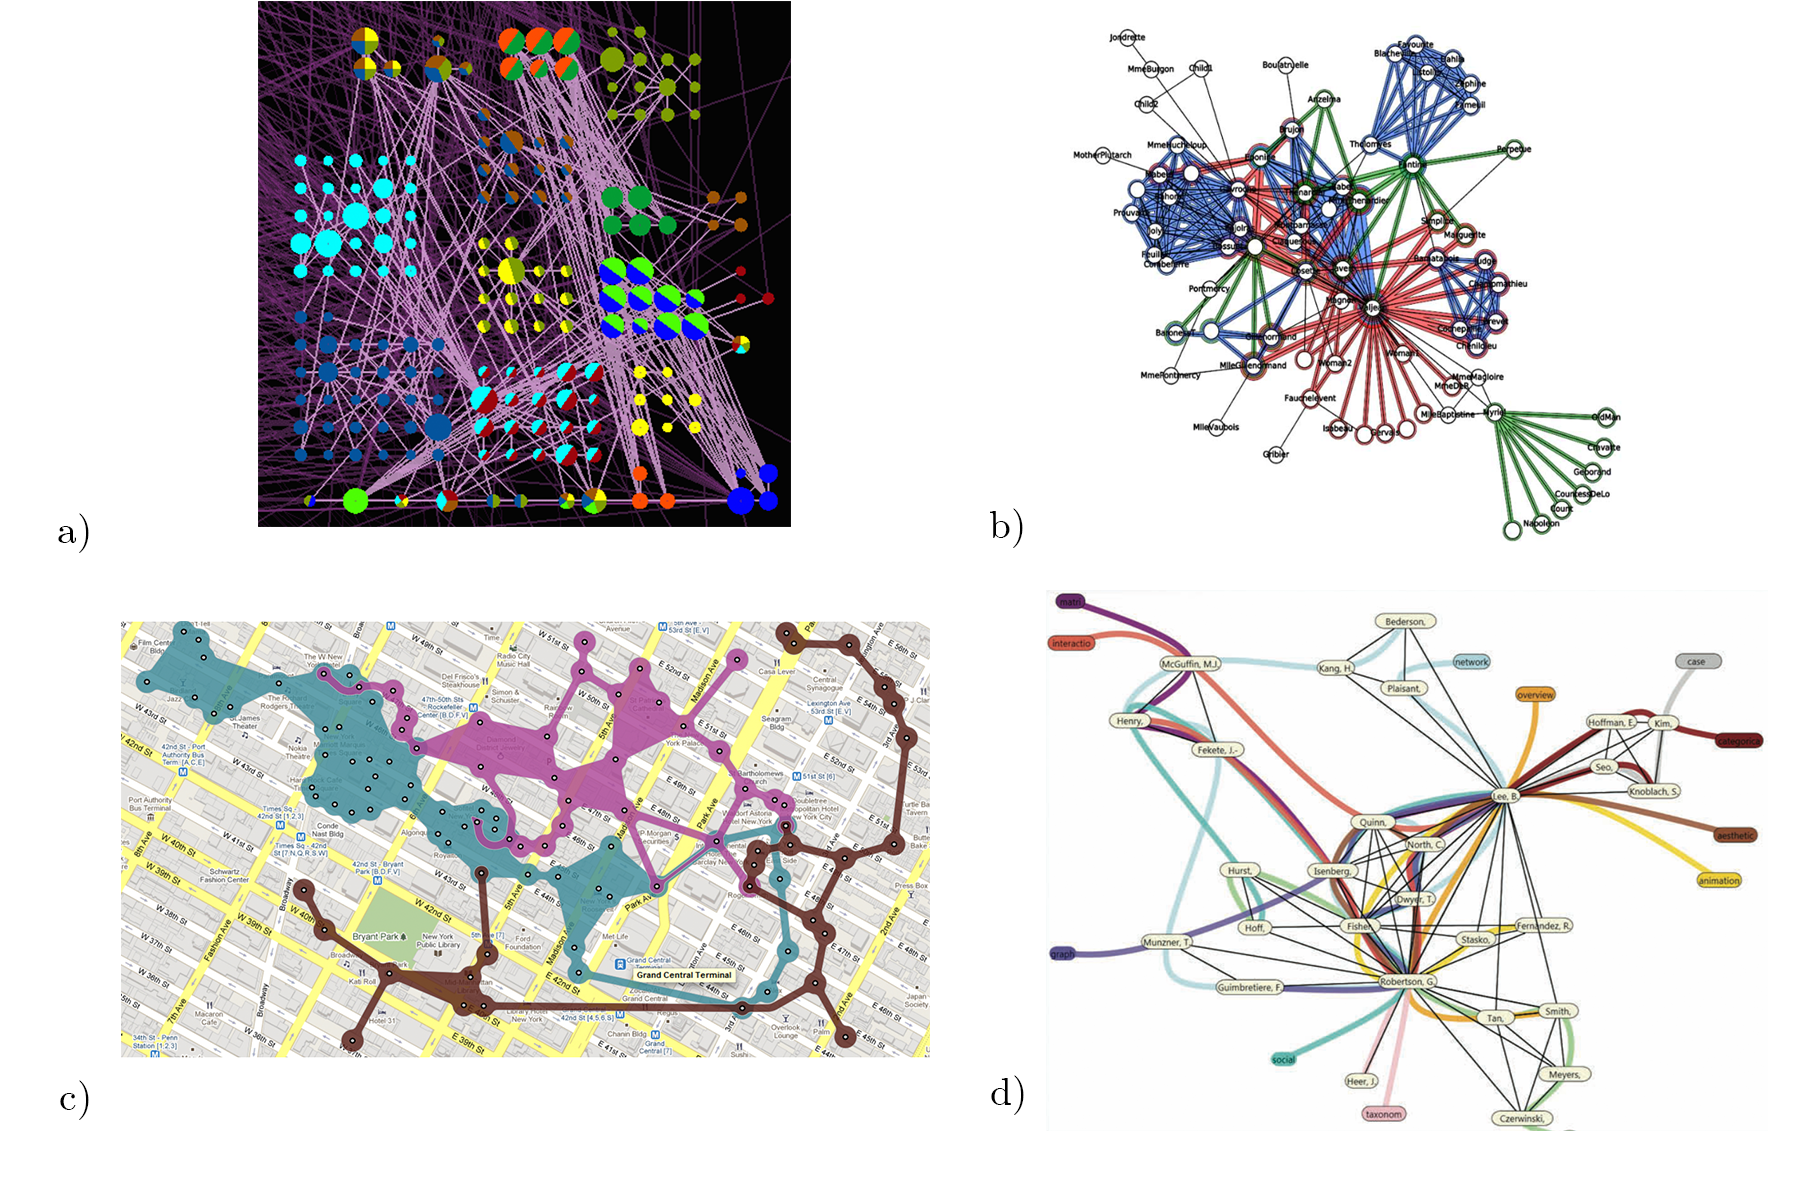
\includegraphics[height=4.1in]{figures/set}
  \caption{Techniques for representing categories in graph structures: \textbf{a)} Each node is divided into multiple fans colored accordingly to its category \textbf{b)} Nodes and edges have colored contours indicating their set membership \textbf{c)} KelpFusion~\cite{meulemans2013kelpfusion} \textbf{d)} LineSets~\cite{linesets}}
  \label{fig:tree}
\end{figure*}   

As mentioned earlier in the discussion of Requirement \ref{req:hierarchy}, pathways are often deeply hierarchical. As mentioned in Requirement \ref{req:hierarchy}, a pathway usually contains multiple sub-pathways, and a protein complex can represent a are often nested hierarchy of constituent proteins. Conventional representations of hierarchical structures with tree diagrams are prone to visual clutter and poor readability as the amount of leaves and the depth of the tree increases. For this reason, different visualization techniques have been developed to efficiently represent complex hierarchical structures.

A \textit{Radial View} is a tree diagram that uses a circular layout in an attempt to more efficient use of a two-dimensional space. With deeply nested trees, a \emph{Radial View} can suffer from the same issues seen with more ``traditional'' tree diagrams. An alternative representation is seen in the \textit{H-tree} layout, which positions nodes by using only orthogonal and perpendicular links, which helps eliminate edge crossings and optimize space. 

\textit{Circle Packing} \cite{stephenson2005introduction} is a technique which presents hierarchical elements as nested circles. This technique provides an efficient overview of a tree structure, however it may be difficult to adapt to more complex and deeply-nested trees. In terms of biological pathways, circle packing layouts may be useful for the understanding of hierarchial structures such as proteins that are nested within complexes, as in Requirement \ref{req:hierarchy}. However, a pathway might contain complexes with hundreds of proteins and dozens of sub-complexes. Circle Packing layouts also present a challenge when it comes to readable labels (Requirement \ref{req:labeling}). Furthermore, understanding the path through a hierarchy from the root node to to a leaf element is challenging with a circle packing layout.

Another representation of hierarchical structure is the \textit{Tree Map}. A tree map places components within rectangles with areas proportional to some given metric. This technique is popular in representing, for example, the memory usage in hard drive, but it may have only limited utility in representing biological pathway data. The spactial organization of a \textit{Tree Map} enables an intuitive understanding of the organization of a structure, but is very difficult to parse when a tree is more than two or three levels deep.

Figure~\ref{fig:tree} compares ``traditional'' tree diagrams to alternative techniques.

\subsection{Matrix-Based Techniques}

Matrix representations act as an alternative to node-link diagrams in representing graphs. Matrix representations excel in their ability to show densely connected graphs while minimizing visual clutter.

Matrix representations present a significant challenge for pathway data, as paths connecting more than two entities can be very difficult to follow. However, matrix views may be an important alternative view of very densely connected biological pathways, such as with large gene regulatory networks.

\section{Tools}

\begin{table*}[htb]
 \centering
\caption{Comparison between the requirements implemented in popular tools for pathway visualization}


\bgroup
\def\arraystretch{1.8}

      \begin{tabular}{  l | c c c c c c c c c c c c c c c c}
      \hline
            \textbf{Tools}&R1&R2&R3&R4 & R5 & R6& R7 & R8 & R8 & R9 & R10 & R11 & R12 & R13 & R14 & R15\\[2ex]\hline 
            Entourage  & \checkmark &\checkmark &\checkmark &\checkmark &\checkmark &   &\checkmark &\checkmark &\checkmark &\checkmark &\checkmark &\checkmark  &   &   &\checkmark &  \checkmark \\
            Reactome &   \checkmark &\checkmark &\checkmark &\checkmark &   &\checkmark &\checkmark &\checkmark &\checkmark &   &\checkmark &   &\checkmark &   &\checkmark &     \\
            VisAnt &     \checkmark &\checkmark &\checkmark &   &\checkmark &   &\checkmark &\checkmark &   &\checkmark &\checkmark &\checkmark &   &   &\checkmark &     \\
            VidaPad &    \checkmark &\checkmark &\checkmark &   &\checkmark &   &   &\checkmark &   &   &\checkmark &   &   &   &\checkmark &     \\
            ChiBe &      \checkmark &\checkmark &\checkmark &\checkmark &   &   &\checkmark &\checkmark &   &\checkmark &\checkmark &\checkmark &   &   &   &     \\
            BioFabric &  \checkmark &   &   &   &   &   &   &   &   &\checkmark &   &\checkmark &   &   &   &     \\
            MetaViz &    \checkmark &\checkmark &\checkmark &   &   &   &   &\checkmark &   &\checkmark &   &\checkmark &   &   &   &     \\
         

        \hline
        
      \end{tabular}
      }
      \label{table:discussion}
\end{table*}

In this section we examine and compare several existing tools for the visualization of biological pathways. Particular attention is given to which requirements detailed in Section~\ref{sec:requirements} are implemented in each tool. Table~\ref{table:discussion} summarizes these relationships.

Broadly speaking, current tools make use of one of three primary visual representations: node-link diagrams, node-link diagrams with compound nodes, and adjacency matrices. We look at \textit{Entourage}~\cite{Lex2013entourage}, \textit{Reactome Pathway Browser}~\cite{croft2014reactome}, \textit{VisAnt}~\cite{hu2004visant}, \textit{MetaViz}~\cite{bourqui2007metabolic} and \textit{VitaPad}~\cite{holford2005vitapad}, each of which leverages a traditional node-link diagram. 

\emph{ChiBE}~\cite{Babur2010chibe} is notable for being one of the first pathway visualization tools to employ \emph{compound nodes}, which can contain either the proteins contained within a complex, or can indicate the cellular location of many pathway components. \emph{ChiBE} provides a basic pannable and zoomable view of a pathway, and includes the ability to display node details on demand through user interaction. Although certain limited analytical functions are available, \emph{ChiBE} is more well-suited to the construction or \emph{curation} of pathways, rather than to insightful pathway analysis.

\textit{Reactome Pathway Browser} is a tool for visualizing pathway diagrams included in the \textit{Reactome} database. It offers basic navigation and limited interactivity. It presents a fixed layout and does not enable the layering of additional meta-data in the same representation. It makes use of multiple panels to enable the inspection of the structure of complexes and to view data from empirical analyses. The \textit{Reactome Pathway Browser} does not enable the simultaneous visualization of multiple pathways but, given a component, it allows the user to navigate through related pathways.

\emph{Entourage}~\cite{Lex2013entourage} is a component of the \emph{Caleydo}~\cite{Lex2010caleydo} framework that displays relationships between proteins and other gene products across multiple pathways. To this end it employs a novel algorithm that extracts \emph{contextual pathways} from larger pathways. Contextual subsets show small portions of a pathway that contain selected proteins of interest. Because the display size of each contextual subset is relatively small, many can be displayed at once, which allows \emph{Entourage} to provide linked views of several pathways that share certain proteins of interest (see Figure~\ref{fig:entourage}). Multiple pathways and sub-pathways are represented in isolated views, which preserves the pathway structure but introduces node redundancy. Links connect proteins or complexes that are shared across pathways, and unless requested by user interaction, these links are reduced to partial ``stubs'' in order to reduce visual clutter. The \textit{Bubble Set} technique is used to highlight selected pathways and visual links are used to connect nodes that are actually the same node.

\emph{Entourage} also allows for the display of both pharmacological and genomic data related to selected gene products that span multiple pathways. Combining functional data with multiple pathway views makes \emph{Entourage} a powerful tool for molecular genomics research.

\begin{figure*}[htb]
  \centering
  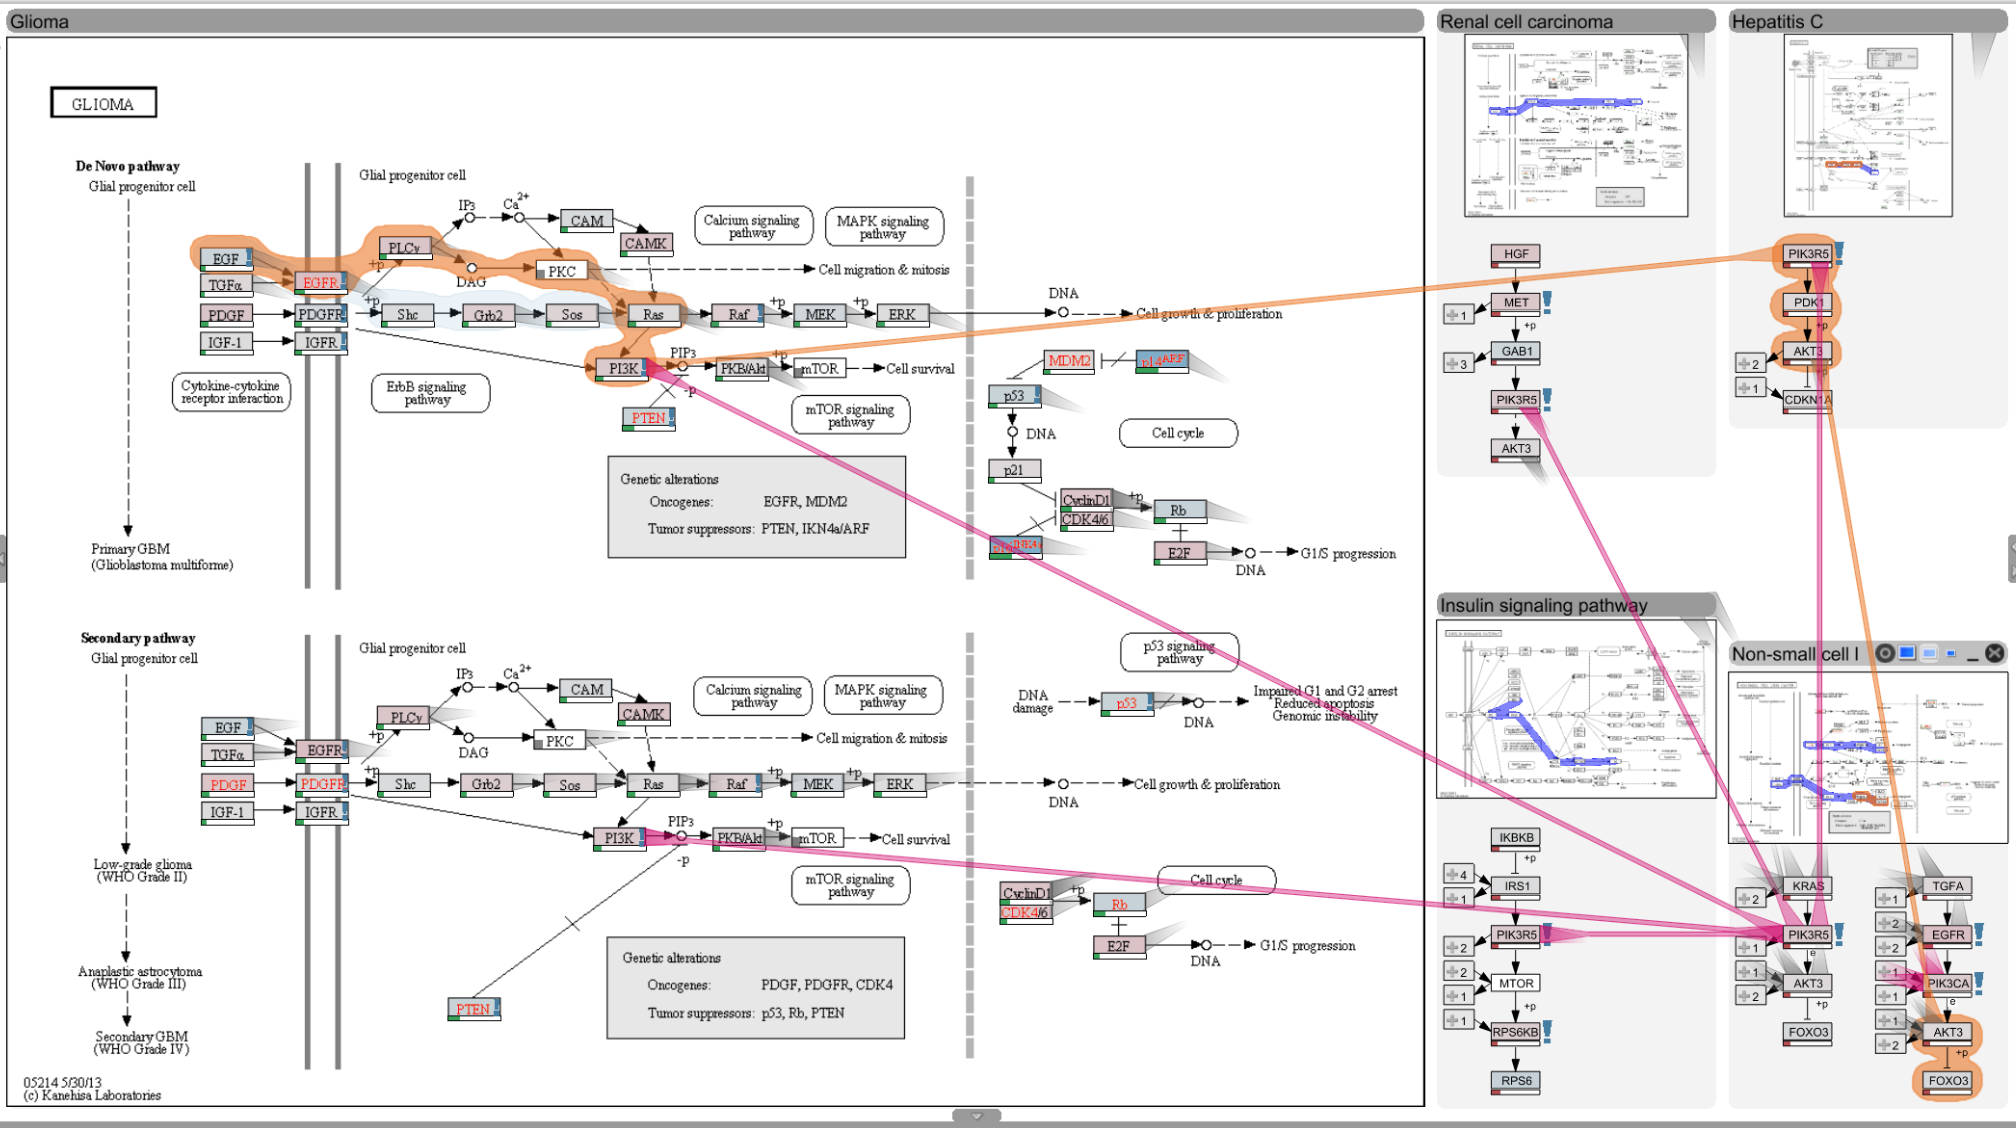
\includegraphics[width=\linewidth]{figures/entourage}
  \caption{\label{fig:entourage} A view of \emph{Entourage} showing links between a larger ``focus pathway'' and several ``context pathways.'' From~\cite{Lex2013entourage}}
\end{figure*}

Furthermore, both \textit{Entourage} and \textit{Reactome Pathway Browser} enable the user to integrate experimental data. \textit{Entourage} prefers to visualize the experiment information as side panels, whereas \textit{Reactome} combine the path visualization with additional visual encoding to show gene expression and other values (Fig~\ref{fig:reactome})

Other tools implement techniques that enable the representation of multiple pathways in the same view, such as \textit{MetaViz}. \textit{MetaViz} visualizes multiple metabolic pathways simultaneously, which allows topological analysis and avoids the duplication of biological components. This method offers different visual layouts depending on the pathway that the user wishes to focus on. The desired pathway will follow a representation which flows from the top to the bottom accordingly the topological ordering of components.

\begin{figure*}[t]
  \centering
  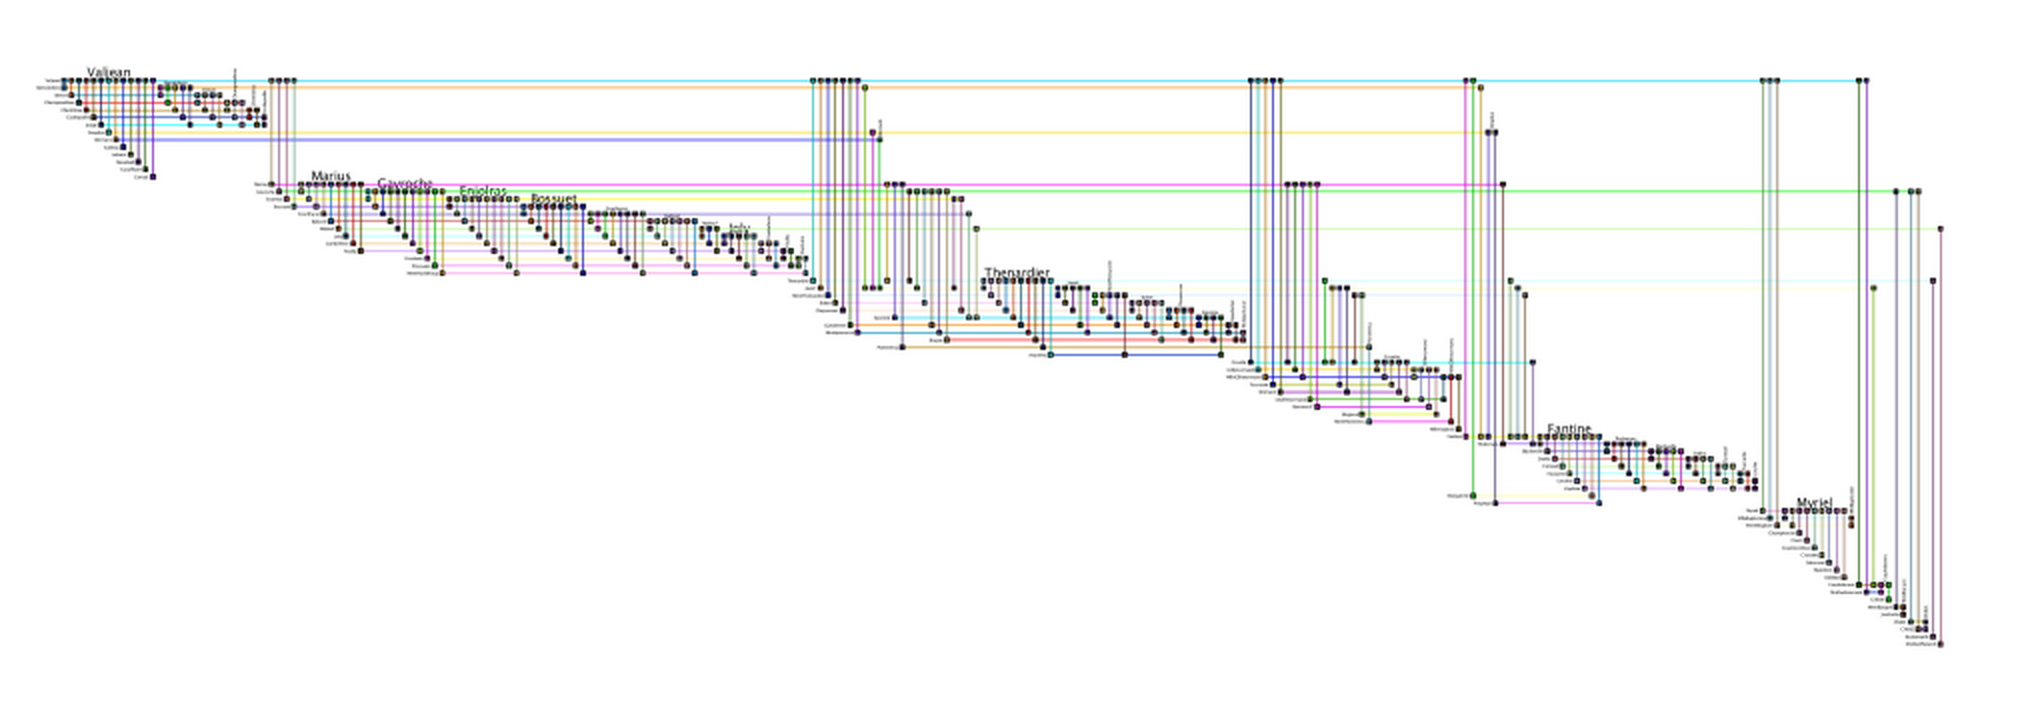
\includegraphics[height=2.5in]{figures/biofabric}
  \caption{Visualizing hundreds of nodes and links with \emph{Biofabric}. Image from~\cite{Longabaugh2012biofabric}}
  \label{fig:biofabric}
\end{figure*}

\begin{figure}[h]
  \centering
  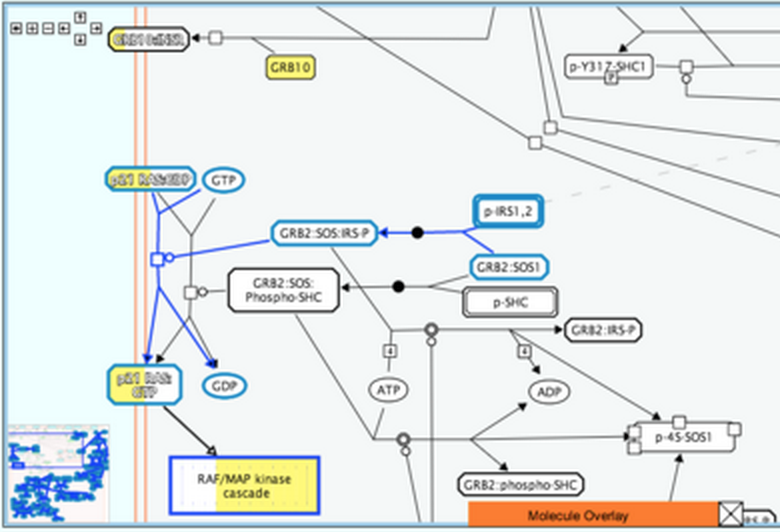
\includegraphics[height=2in]{figures/reactome}
  \caption{Visualizing gene expression data with \emph{Reactome Pathway Browser}. Image from ~\cite{reactome}}
  \label{fig:reactome}
\end{figure}

\textit{BioFabric}~\cite{Longabaugh2012biofabric} also enables the exploration of large biological networks composed by multiple pathways without replicating nodes. This novel tool is meant to visualize extremely large networks composed of thousands of nodes. This tool is designed specifically for genetic interaction networks, and thus it does not implement any pathways-specific tasks. However, this tools can import SIF files which are commonly used for pathway visualizations. Figure~\ref{fig:biofabric} represents a network with hundreds of nodes and links. Elements are represented with horizontal lines, and links with vertical lines. Although this tools is considerably less intuitive than node-link diagram, it enables the representation of large networks without a loss of detail.

\textit{VisAnt}~\cite{hu2004visant} enables a wide range of exploratory questions and tasks related to network topology. Tasks include finding shortest paths between two nodes \cite{hu2013visant} as well as detection of clusters of dense nodes. The positions of the nodes in the graph are computed with a relaxing layout algorithm which models the network as a set of physical entities. This algorithm builds a graphical representation that organizes the graph by the density of the connections between clusters of nodes. Diagrams can include abstract nodes that extend beyond the typical components found in a biological pathway. Diseases, genes, therapies, and drugs are presented together in the same graph with more ``typical'' pathway components such as proteins and complexes. \textit{VisAnt} permits a dynamic exploration of a biological network composed by multiple pathways. However, if more than one pathway includes the same node, multiple instances of the node will be present in the representation. Furthermore, layouts are restricted to either force-directed or hub-spoke algorithms.

Although in the majority of available tools the visual encoding of a biological network remains limited to the conventional graph representations, pathway analysis tools often decorate node-link representations with experimental data or additional meta-data. \textit{VitaPad} \cite{holford2005vitapad}, for example, allows the user to incorporate micro-array data into pathways and offers a flexible visualization.

\section{Future Work}

Design an effective and compresensive visualization platform for biological pathways presents a variety of challenges. The techniques reviewed in this paper offer solutions to these challenges, some of which have been implemented in existing pathway analysis tools. However, the construction of a comprehensive analytics platform that implements a large majority of the requirements listed in our analysis has yet to be realized. Here, we identify several ``front-lines'' of improvement.

\subsection{User Interactions and Visual Encodings}

Comprehensive tools should provide highly interactive layouts and visual encodings. Some tools still present fixed layouts and implement only limited interactivity. These tools might improve in the near future by implementing more well-designed user interactions and functionality. However, the majority of pathway representations are still tied to conventional node-link representations.The visual encoding of node-link diagrams can be augmented with additional techniques, such as bubble-sets layered on a graph to provide categorical information. Furthermore, techniques such as \textit{edge bundling} or \textit{fisheye distortion} that can be easily embedded in graph representations should be included in pathway visualization tools.

\subsection{Web-Based Data Integration}

The prevalence of large online databases with comprehensive APIs makes web-based tools attractive solutions for biological pathway analysis platforms. Online tools also improve accessibility. For instance, one of the researchers we interviewed, QW, used \emph{Ingenuity Pathway Analysis}~\cite{Kramer2013ipa-causal} to present her findings, but was frustrated by the limitations of the desktop application

\emph{KEGG} and \emph{Reactome}, while providing online database access, both offer very basic tools pathway visualization. Our interviews with domain experts revealed, for example, that researchers in bioinformatics usually need to merge pathway information from different sources in order to produce a higher quality pathway. Some tools enable the user to import standard formats (which can be exported from databases) or to import data from a hyperlink. However, modern tools should enable the exploration of the huge amount of pathway data contained within online databases. Cutting edge tools will allow participants to actively search online databases and to assemble complex pathways based on network queries. High quality data representation must be supported by high quality data.

\subsection{Embracing Abstract Visualization Techniques}

Nearly every tool in this review uses some type of node-link diagram. The few exceptions are matrix based (\emph{BioFabric} and \emph{Compressed Adjacency Matrices}) but they can only be used for very specific types of networks, and they do not provide solutions relevant to pathway data specifically, such as discovering paths between two proteins of interest. Further work should be done to explore the possible benefits of abstract representations, as almost every tool in this review relies on automatic or human-curated node-link diagrams.

The visual representation of pathways has until recently been confined to static representations that lack substantial user interactions. Current pathway visualization tools rely almost entirely on ``traditional'' node link diagrams, and only a few of the techniques detailed in Section~\ref{sec:representation} have been implemented in pathway visualization tools. The adoption of new representations could lead to more robust analysis platforms and inspire creative avenues of research.

\subsection{Visualizing Uncertainty}

Especially considering our feedback from domain experts, tools generally do not attempt to visualize the ``uncertainty'' behind a connection in a pathway, as expressed by the first domain expert. This is a challenging task, as even the definition of ``uncertainty'' may be difficult to operationalize. However, data formats such as \emph{BioPAX} do have robust support for citations, allowing published references to be connected to entities and relationships within a pathway. A tool that could effectively encode ``uncertainty data'' into a visualization may be very valuable to systems researchers who work with the results of hundereds or thousands of separate publications.

\subsection{Inference and Simulation}

Being able to situate some hypothetical new reaction within the context of a pathway database would likely be a valuable tool to these domain researchers. This avenue is also closely related to \emph{causal anaylsis}, which as of this writing is only performed within the \emph{Ingenuity Pathway Analysis}~\cite{Kramer2013ipa-causal} tool. Effective visualization of causal relationships -- and especially \emph{potential} relationships that have yet to be confirmed -- could produce exciting new avenues of research for molecular biologists.

\section{Conclusion}

While a wide variety of pathway visualization tools exist, there is still plenty of room for innovative platform development. Many tools tend to greatly overlap each other with respect to the analytical tasks available, and attempts to address the most challenging aspects of pathway data analysis are few and far between. Having a detailed understanding of the tasks performed by researchers who work with pathway data is essential to the development of effective pathway visual analytics platforms. With the increasing popularity of web-based tools that integrate multiple databases and reduce accessibility costs, and with a number of innovative techniques for the vizualization of complex, hierarchial data, there is great potential for the development of innovative and useful platforms for complex biological pathway analytics.

\bibliographystyle{abbrv}
%%use following if all content of bibtex file should be shown
%\nocite{*}
\bibliography{references}
\end{document}

